\documentclass{article}\usepackage[]{graphicx}\usepackage[]{color}
%% maxwidth is the original width if it is less than linewidth
%% otherwise use linewidth (to make sure the graphics do not exceed the margin)
\makeatletter
\def\maxwidth{ %
  \ifdim\Gin@nat@width>\linewidth
    \linewidth
  \else
    \Gin@nat@width
  \fi
}
\makeatother

\definecolor{fgcolor}{rgb}{0.345, 0.345, 0.345}
\newcommand{\hlnum}[1]{\textcolor[rgb]{0.686,0.059,0.569}{#1}}%
\newcommand{\hlstr}[1]{\textcolor[rgb]{0.192,0.494,0.8}{#1}}%
\newcommand{\hlcom}[1]{\textcolor[rgb]{0.678,0.584,0.686}{\textit{#1}}}%
\newcommand{\hlopt}[1]{\textcolor[rgb]{0,0,0}{#1}}%
\newcommand{\hlstd}[1]{\textcolor[rgb]{0.345,0.345,0.345}{#1}}%
\newcommand{\hlkwa}[1]{\textcolor[rgb]{0.161,0.373,0.58}{\textbf{#1}}}%
\newcommand{\hlkwb}[1]{\textcolor[rgb]{0.69,0.353,0.396}{#1}}%
\newcommand{\hlkwc}[1]{\textcolor[rgb]{0.333,0.667,0.333}{#1}}%
\newcommand{\hlkwd}[1]{\textcolor[rgb]{0.737,0.353,0.396}{\textbf{#1}}}%
\let\hlipl\hlkwb

\usepackage{framed}
\makeatletter
\newenvironment{kframe}{%
 \def\at@end@of@kframe{}%
 \ifinner\ifhmode%
  \def\at@end@of@kframe{\end{minipage}}%
  \begin{minipage}{\columnwidth}%
 \fi\fi%
 \def\FrameCommand##1{\hskip\@totalleftmargin \hskip-\fboxsep
 \colorbox{shadecolor}{##1}\hskip-\fboxsep
     % There is no \\@totalrightmargin, so:
     \hskip-\linewidth \hskip-\@totalleftmargin \hskip\columnwidth}%
 \MakeFramed {\advance\hsize-\width
   \@totalleftmargin\z@ \linewidth\hsize
   \@setminipage}}%
 {\par\unskip\endMakeFramed%
 \at@end@of@kframe}
\makeatother

\definecolor{shadecolor}{rgb}{.97, .97, .97}
\definecolor{messagecolor}{rgb}{0, 0, 0}
\definecolor{warningcolor}{rgb}{1, 0, 1}
\definecolor{errorcolor}{rgb}{1, 0, 0}
\newenvironment{knitrout}{}{} % an empty environment to be redefined in TeX

\usepackage{alltt}

\usepackage{amsmath}
\IfFileExists{upquote.sty}{\usepackage{upquote}}{}
\begin{document}

\section{Chapter 3}

\begin{enumerate}

  \item Since $P\left(A_1 \cap A_2\right) = 0.64 = (0.8)(0.8) = P\left(A_1\right)P\left(A_2\right)$, we can conclude that $A_1$ and $A_2$ are independent; hence, the answer is (c).
  
  \item
  
  \begin{enumerate}
  
    \item $P\left(A \cap B\right) = P\left(B \cap A\right) = P\left(B|A\right) = (0.95)(0.05) = 0.0475$.
    
    \item $P\left(B\right) = P\left(B \cap A\right) + P\left(B \cap A^c\right) = 0.0475 + (.03)(1 - 0.05) = 0.076$.
    
    \item $P\left(A|B\right) = P\left(A \cap B\right) / P\left(B\right) = 0.0475 / 0.076 = 0.625$.
  
  \end{enumerate}
  
  \item Let $A$ be the event that an adult gets the flu and let $B$ be the event that an adult gets the flu shot. 
  
  \begin{enumerate}
  
    \item $P\left(A \cap B\right) = P\left(A|B\right)P\left(B\right) = (0.1)(0.42) = 0.042$.
    
    \item $P\left(A\right) = P\left(A \cap B\right) + P\left(A \cap B^c\right) = 0.042 + (0.7)(1 - 0.42) = 0.448$.
    
  \end{enumerate}
  
  \item Let $X$ denote the number of people who have asthma. Then $X \sim Binomial\left(n = 50, p = 0.2\right)$. (Think about why!)
  
  \begin{enumerate}
  
    \item $P\left(X = 19\right) = \binom{50}{19}(0.2)^{19}(0.8)^{50-19} = \approx 0.001579$.
    
    \item The standard deviation is $\sigma = \sqrt{np\left(1 - p\right)} = \sqrt{(50)(0.2)(0.8)} = 2.828427$ and the mean/expected value is $\mu = np = (50)(0.2) = 10$. Hence, the $z$-score is $\left(19 - 10\right) / 2.828427 \approx 3.181981$ which implies that 19 is a little over three standard deviations above the mean.
    
    \item Using the empirical rule, we have that $P\left(X \ge 19\right) \approx P\left(X \ge \mu + 3\sigma\right) \approx \left(1 - 0.997\right) / 2 = 0.003 / 2 = 0.0015$. (Draw a picture!). The exact answer is 
\begin{knitrout}
\definecolor{shadecolor}{rgb}{0.969, 0.969, 0.969}\color{fgcolor}\begin{kframe}
\begin{alltt}
\hlnum{1} \hlopt{-} \hlkwd{pbinom}\hlstd{(}\hlnum{18}\hlstd{,} \hlkwc{size} \hlstd{=} \hlnum{50}\hlstd{,} \hlkwc{prob} \hlstd{=} \hlnum{0.2}\hlstd{)}
\end{alltt}
\begin{verbatim}
## [1] 0.002511203
\end{verbatim}
\end{kframe}
\end{knitrout}
    
  \end{enumerate}
  
  \item $E\left[X\right] = \sum_{r = 1}^3 rP\left(X = r\right) = (1)\left(1/3\right) + (2)\left(1/3\right) + (3)\left(1/3\right) = 2$ envelopes.
  
  \item 
  
  \begin{enumerate}
  
    \item $E\left[X\right] = \mu = \sum_{r = 0}^4 rP\left(X = r\right) = (0)(0.2) + (1)(0.3) + (2)(0.3) + (3)(0.1) + (4)(0.1) = 1.6$ egg masses.
    
    \item $Var\left[X\right] = \sum_{r = 0}^4 \left(r - \mu\right) ^ 2 P\left(X = r\right) = \left(0 - 1.6\right)^2(0.2) + \left(1 - 1.6\right)^2(0.3) + \left(2 - 1.6\right)^2(0.3) + \left(3 - 1.6\right)^2(0.1) + \left(4 - 1.6\right)^2(0.1) = 1.44$. Hence, the standard deviation is $\sqrt{1.44} = 1.2$ egg masses.
  
  \end{enumerate}
  
  \item Let $A$ be the event that a subject is taking the drug (then $A^c$ is the event that the subject is taking the placebo) and let $B$ be the event that a subject improves.
  
  \begin{enumerate}
  
    \item $P\left(B \cap A\right) = P\left(B | A\right)P\left(A\right) = (0.6)(0.5) = 0.3$.
    \item $P\left(B\right) = P\left(B \cap A\right) + P\left(B \cap A^c\right) = 0.3 + (0.35)(0.5) = 0.475$.
  
  \end{enumerate}
  
  \item Let $Y$ be a random variable denoting the number of chickens out of 20 with the bird flu. It then follows that $Y \sim Binomial\left(n = 20, p = 0.1\right)$.
  
  \begin{enumerate}
  
    \item $P\left(Y = 5\right) = \binom{20}{5}(0.1)^5(0.9)^15 = (15504)\left(10^{-5}\right)(0.2058911) \approx 0.031921$.
    
    \item $E\left[Y\right] = np = (20)(0.1) = 2$ chickens.
    
    \item $\sqrt{Var\left[Y\right]} = \sqrt{np(1-p)} = \sqrt{(20)(0.1)(0.9)} \approx 1.3416$ chickens.
  
  \end{enumerate}
  
  \item Let $X$ be a random variable denoting the number of frog eggs that hatch out of 100. Then, $X \sim Binomial\left(n = 100, p = 0.87\right)$. (Since the frog eggs hatch independently of each other!)
  
  \begin{enumerate}
  
    \item $P\left(X = 80\right) = \binom{100}{80}(0.87)^{80}(0.13)^{20} \approx 0.01477606$. You should be able to do this with a calculator, but in R we would just use
\begin{knitrout}
\definecolor{shadecolor}{rgb}{0.969, 0.969, 0.969}\color{fgcolor}\begin{kframe}
\begin{alltt}
\hlkwd{dbinom}\hlstd{(}\hlnum{80}\hlstd{,} \hlkwc{size} \hlstd{=} \hlnum{100}\hlstd{,} \hlkwc{prob} \hlstd{=} \hlnum{0.87}\hlstd{)}
\end{alltt}
\begin{verbatim}
## [1] 0.01477606
\end{verbatim}
\end{kframe}
\end{knitrout}
  
    \item For a binomial random variable, $E\left[X\right] = np = (100)(0.87) = 87$ eggs.
    
    \item To use the empirical rule, we must first calculate the standard deviation of $X$. The stahndard deviation of a binomial random variable is given by $\sqrt{Var\left[X\right]} = \sqrt{np(1-p)} = \sqrt{3.31} = 3.363034$. Computing the $z$-score yields
    \begin{equation*}
      Z = \frac{77 - 87}{3.363034} = -2.973505 \approx -3.
    \end{equation*}
  In other words, 77 eggs is about three standard deviations below the mean. So, $P\left(X \le 77\right) \approx$ the probability of being three or more standard deviations below the mean $\approx 0.003 / 2 = 0.0015$.

  \end{enumerate}

  \item 
  
  \begin{enumerate}
  
    \item $\binom{20}{5} = \frac{20!}{5!(20 - 5)!} = \frac{(20)(19)(18)(17)(16)(15!)}{5!(15!)} = 15504$.
    
    \item $P\left(X = 0\right) = \binom{5}{0}\left(7/20\right)^0(1 - 7/20)^5 = 0.116$.
  
  \end{enumerate}
  
  \item Let $X$ be a random variable that represents the number of white croaker fish with high mercury levels out of $n = 100$. It follows that $X \sim Binomial\left(n = 100, p = 0.4\right)$.
  
  \begin{enumerate}
  
    \item $P\left(X = 100\right) = (0.4)^100 \approx 1.6069 \times 10^{-40}$.
    
    \item $P\left(X = 45\right) = \binom{100}{45}(0.4)^{45}(1 - 0.4)^{55} = 0.0478$.
    
    \item $E\left[X\right] = np = (100)(0.4) = 40$ fish and $\sqrt{Var\left[X\right]} = \sqrt{np(1-p)} = \sqrt{(100)(0.4)(0.6)} = 4.898979$ fish.
    
    \item $P\left(X \ge 55\right) = 1 - P\left(X \le 54\right) = 1 - \left[P\left(X = 0\right) + P\left(X = 1\right) + \dots P\left(X = 54\right)\right]$. In R, we get
\begin{knitrout}
\definecolor{shadecolor}{rgb}{0.969, 0.969, 0.969}\color{fgcolor}\begin{kframe}
\begin{alltt}
\hlnum{1} \hlopt{-} \hlkwd{pbinom}\hlstd{(}\hlnum{54}\hlstd{,} \hlkwc{size} \hlstd{=} \hlnum{100}\hlstd{,} \hlkwc{prob}  \hlstd{=} \hlnum{0.4}\hlstd{)}
\end{alltt}
\begin{verbatim}
## [1] 0.001710927
\end{verbatim}
\end{kframe}
\end{knitrout}
  
  \end{enumerate}
  
\end{enumerate}




\section{Chapter 4}

\begin{enumerate}
  \item No (it looks bimodal).
  \item The best answer is (d); bimodal.
  \item The population might consist of both males and females, and each of these subpopulations probably has its own mean.
  \item The best answer is (a); 31.
  \item The best answer is (c); 0.22.
  \item The best answer is (e); 0.94.
  \item It will remain the same. Go back to the properties about correlation and linear transformations!
  \item The best answer is (d); 0.27.
  \item The best answer is (d); 0.58.
  \item Use the fact that $X \sim N\left(\mu = 5.28, \sigma = 0.4\right)$.
  \begin{enumerate}
    \item \begin{align*}
             P\left(X > 5.4\right) &= 1 - P\left(X \le 5.4 \right) \\
             &= 1 - P\left(\frac{X - 5.28}{0.4} < \frac{5.4 - 5.28}{0.4}\right) \\
             &= 1 - P\left(Z < \frac{5.4 - 5.28}{0.4}\right) \\
             &= 1 - P\left(Z < 0.3\right) \\
             &= 1 - \Phi\left(0.3\right)
          \end{align*}
          In R, we get
\begin{knitrout}
\definecolor{shadecolor}{rgb}{0.969, 0.969, 0.969}\color{fgcolor}\begin{kframe}
\begin{alltt}
\hlnum{1} \hlopt{-} \hlkwd{pnorm}\hlstd{(}\hlnum{0.3}\hlstd{)}
\end{alltt}
\begin{verbatim}
## [1] 0.3820886
\end{verbatim}
\end{kframe}
\end{knitrout}
    \item \begin{align*}
             P\left(5 < X < 6\right) &= P\left(X < 6 \right) - P\left(X < 5 \right) \\
             &= P\left(\frac{X - 5.28}{0.4} < \frac{6 - 5.28}{0.4}\right) - P\left(\frac{X - 5.28}{0.4} < \frac{5 - 5.28}{0.4}\right) \\
             &= P\left(Z < \frac{6 - 5.28}{0.4}\right) - P\left(Z < \frac{5 - 5.28}{0.4}\right) \\
             &= P\left(Z < 1.8\right) - P\left(Z < -0.7\right) \\
             &= \Phi\left(1.8\right) - \Phi\left(-0.7\right)
          \end{align*}
          In R, we get
\begin{knitrout}
\definecolor{shadecolor}{rgb}{0.969, 0.969, 0.969}\color{fgcolor}\begin{kframe}
\begin{alltt}
\hlkwd{pnorm}\hlstd{(}\hlnum{1.8}\hlstd{)} \hlopt{-} \hlkwd{pnorm}\hlstd{(}\hlopt{-}\hlnum{0.7}\hlstd{)}
\end{alltt}
\begin{verbatim}
## [1] 0.722106
\end{verbatim}
\end{kframe}
\end{knitrout}
    \item The general formula for the $p$-th percentile, denoted $x_p$, of a normal distribution with mean $\mu$ and standard deviation $\sigma$ is 
    \begin{equation*}
      x_p = \mu + \sigma z_p, 
    \end{equation*}
    where $z_p$ is the $p$-th percentile of a standard normal distribution (which we can obtain using \texttt{qnorm(p)} in R). Hence, the 95-th percentile is $x_{0.95} = 5.28 + 0.4 z_{0.95}$. Using \texttt{qnorm(0.95)} in R, we obtain $x_{0.95} = 5.28 + 0.4\left(1.644854\right) = 5.937941$.
    \item Since the data are a random sample from a normal distribution, we know that the sample mean also has a normal distribution; in particular, $\bar{X} \sim N\left(\mu = 5.28, \sigma = 0.4 / \sqrt{50}\right)$. Hence,
    \begin{align*}
      P\left(\bar{X} > 5.4\right) &= 1 - P\left(\bar{X} \le 5.4 \right) \\
        &= 1 - P\left(\frac{\bar{X} - 5.28}{0.4 / \sqrt{50}} < \frac{5.4 - 5.28}{0.4 / \sqrt{50}}\right) \\
        &= 1 - P\left(Z < \frac{5.4 - 5.28}{0.4 / \sqrt{50}}\right) \\
        &= 1 - P\left(Z < 2.12132\right) \\
        &= 1 - \Phi\left(2.12132\right)
    \end{align*}
    In R, we get
\begin{knitrout}
\definecolor{shadecolor}{rgb}{0.969, 0.969, 0.969}\color{fgcolor}\begin{kframe}
\begin{alltt}
\hlnum{1} \hlopt{-} \hlkwd{pnorm}\hlstd{(}\hlnum{2.12132}\hlstd{)}
\end{alltt}
\begin{verbatim}
## [1] 0.01694744
\end{verbatim}
\end{kframe}
\end{knitrout}
  \end{enumerate}
  
  \item Use the fact that $X \sim N\left(\mu = 170, \sigma = 20\right)$.
  \begin{enumerate}
    \item \begin{align*}
             P\left(X > 200\right) &= 1 - P\left(X \le 200\right) \\
             &= 1 - P\left(\frac{X - 170}{20} < \frac{200 - 170}{20}\right) \\
             &= 1 - P\left(Z < \frac{200 - 170}{20}\right) \\
             &= 1 - P\left(Z < 1.5\right) \\
             &= 1 - \Phi\left(1.5\right)
          \end{align*}
          In R, we get
\begin{knitrout}
\definecolor{shadecolor}{rgb}{0.969, 0.969, 0.969}\color{fgcolor}\begin{kframe}
\begin{alltt}
\hlnum{1} \hlopt{-} \hlkwd{pnorm}\hlstd{(}\hlnum{1.5}\hlstd{)}
\end{alltt}
\begin{verbatim}
## [1] 0.0668072
\end{verbatim}
\end{kframe}
\end{knitrout}
    \item Using the fact that $\bar{X} \sim N\left(\mu = 170, \sigma = 20 / \sqrt{20}\right)$, we get
      \begin{align*}
        P\left(\bar{X} > 200\right) &= 1 - P\left(\bar{X} \le 200\right) \\
          &= 1 - P\left(\frac{\bar{X} - 170}{20 / \sqrt{20}} < \frac{200 - 170}{20 / \sqrt{20}}\right) \\
          &= 1 - P\left(Z < \frac{200 - 170}{20 / \sqrt{20}}\right) \\
          &= 1 - P\left(Z < 6.708204\right) \\
          &= 1 - \Phi\left(6.708204\right)
      \end{align*}
      In R, we get
\begin{knitrout}
\definecolor{shadecolor}{rgb}{0.969, 0.969, 0.969}\color{fgcolor}\begin{kframe}
\begin{alltt}
\hlnum{1} \hlopt{-} \hlkwd{pnorm}\hlstd{(}\hlnum{6.708204}\hlstd{)}
\end{alltt}
\begin{verbatim}
## [1] 9.851675e-12
\end{verbatim}
\end{kframe}
\end{knitrout}
      
    \item $x_{0.95} = \mu + \sigma z_{0.95} = 170 + 20 \left(1.644854\right) = 202.8971$ (mg/dL).
    
  \end{enumerate}
  
\end{enumerate}


\section{Chapter 5}

\begin{enumerate}

  \item Using the central limit theorem, $\bar{X} \sim N\left(\mu = 19, \sigma = 7.8 / \sqrt{30}\right)$. So, 
      \begin{align*}
        P\left(\bar{X} > 21.3\right) &= 1 - P\left(\bar{X} \le 21.3\right) \\
          &= 1 - P\left(\frac{\bar{X} - 19}{7.8 / \sqrt{30}} < \frac{21.3 - 19}{7.8 / \sqrt{30}}\right) \\
          &= 1 - P\left(Z < \frac{21.3 - 19}{7.8 / \sqrt{30}}\right) \\
          &= 1 - P\left(Z < 1.615079\right) \\
          &= 1 - \Phi\left(1.615079\right)
      \end{align*}
      In R, we get
\begin{knitrout}
\definecolor{shadecolor}{rgb}{0.969, 0.969, 0.969}\color{fgcolor}\begin{kframe}
\begin{alltt}
\hlnum{1} \hlopt{-} \hlkwd{pnorm}\hlstd{(}\hlnum{1.615079}\hlstd{)}
\end{alltt}
\begin{verbatim}
## [1] 0.05314679
\end{verbatim}
\end{kframe}
\end{knitrout}
      
  \item \begin{enumerate}
          \item Running the R script \texttt{\textbf{maleturtle.R}}, a 99\% confidence interval for the mean carapace length is $\left(106.6246, 120.1254\right)$.
          \item Running the R script \texttt{\textbf{maleturtle.R}}, a 99\% confidence interval for the mean carapace width is $\left(84.23794, 92.34539\right)$.
          \item Based on the plot, it seems reasonable that this sample belongs to the Painted Turtle species (the true mean happens to be captured in the 99\% confidence intervals).
          \item Narrower, since we are decreaing our confidence.
          \item The normal approximation does not seem unreasonable here, but more data is needed to get a clearer picture. In R, try
\begin{knitrout}
\definecolor{shadecolor}{rgb}{0.969, 0.969, 0.969}\color{fgcolor}\begin{kframe}
\begin{alltt}
\hlcom{# Carapace length}
\hlstd{length} \hlkwb{<-} \hlkwd{c}\hlstd{(}\hlnum{93}\hlstd{,} \hlnum{94}\hlstd{,} \hlnum{96}\hlstd{,} \hlnum{101}\hlstd{,} \hlnum{102}\hlstd{,} \hlnum{103}\hlstd{,} \hlnum{104}\hlstd{,} \hlnum{106}\hlstd{,} \hlnum{107}\hlstd{,}
  \hlnum{112}\hlstd{,} \hlnum{113}\hlstd{,} \hlnum{114}\hlstd{,} \hlnum{116}\hlstd{,} \hlnum{117}\hlstd{,} \hlnum{117}\hlstd{,} \hlnum{119}\hlstd{,} \hlnum{120}\hlstd{,} \hlnum{120}\hlstd{,} \hlnum{121}\hlstd{,} \hlnum{125}\hlstd{,}
  \hlnum{127}\hlstd{,} \hlnum{128}\hlstd{,} \hlnum{131}\hlstd{,} \hlnum{135}\hlstd{)}

\hlcom{# Carapce width}
\hlstd{width} \hlkwb{<-} \hlkwd{c}\hlstd{(}\hlnum{74}\hlstd{,} \hlnum{78}\hlstd{,} \hlnum{80}\hlstd{,} \hlnum{84}\hlstd{,} \hlnum{85}\hlstd{,} \hlnum{81}\hlstd{,} \hlnum{83}\hlstd{,} \hlnum{83}\hlstd{,} \hlnum{82}\hlstd{,} \hlnum{89}\hlstd{,} \hlnum{88}\hlstd{,}
  \hlnum{86}\hlstd{,} \hlnum{90}\hlstd{,} \hlnum{90}\hlstd{,} \hlnum{91}\hlstd{,} \hlnum{93}\hlstd{,} \hlnum{89}\hlstd{,} \hlnum{93}\hlstd{,} \hlnum{95}\hlstd{,} \hlnum{93}\hlstd{,} \hlnum{96}\hlstd{,} \hlnum{95}\hlstd{,} \hlnum{95}\hlstd{,} \hlnum{106}\hlstd{)}

\hlcom{# Histograms}
\hlkwd{par}\hlstd{(}\hlkwc{mfrow} \hlstd{=} \hlkwd{c}\hlstd{(}\hlnum{1}\hlstd{,} \hlnum{2}\hlstd{))}
\hlkwd{hist}\hlstd{(length,} \hlkwc{br} \hlstd{=} \hlnum{5}\hlstd{)}
\hlkwd{hist}\hlstd{(width,} \hlkwc{br} \hlstd{=} \hlnum{5}\hlstd{)}
\end{alltt}
\end{kframe}
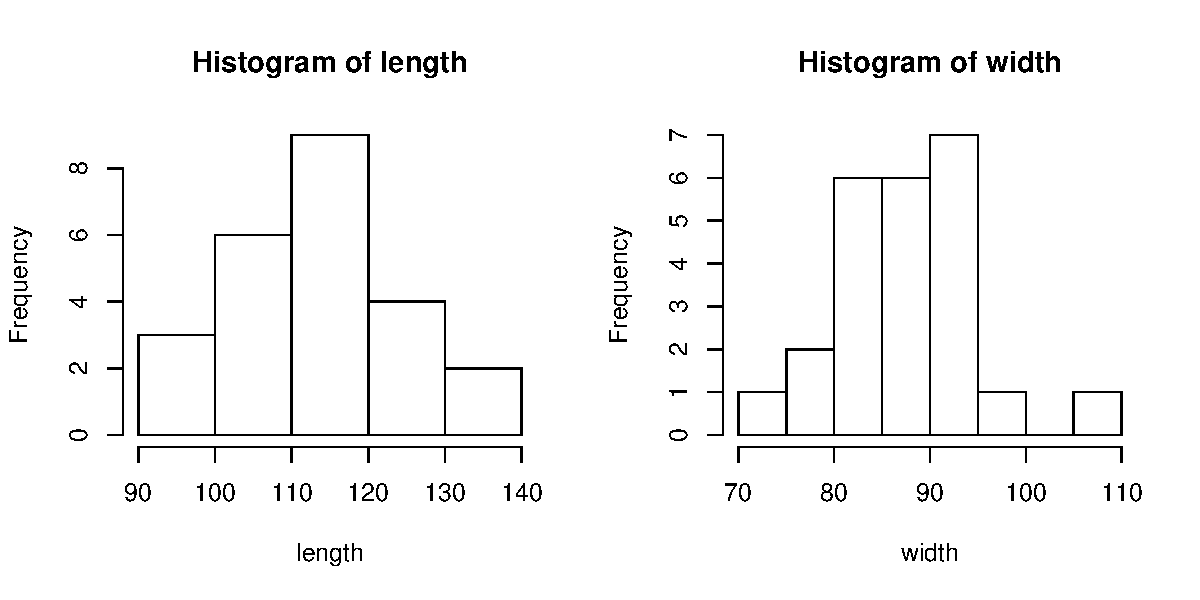
\includegraphics[width=\maxwidth]{figure/unnamed-chunk-10-1} 

\end{knitrout}
        \end{enumerate}
        
  \item In R, you could use
\begin{knitrout}
\definecolor{shadecolor}{rgb}{0.969, 0.969, 0.969}\color{fgcolor}\begin{kframe}
\begin{alltt}
\hlcom{# Path to data set on my laptop}
\hlstd{path} \hlkwb{<-} \hlstr{"C:\textbackslash{}\textbackslash{}Users\textbackslash{}\textbackslash{}greenweb\textbackslash{}\textbackslash{}Desktop\textbackslash{}\textbackslash{}Filing cabinet\textbackslash{}\textbackslash{}STT 6300\textbackslash{}\textbackslash{}Data sets\textbackslash{}\textbackslash{}bodytemp.csv"}

\hlcom{# If you don't know how to find this, then just use: path <- file.choose()}

\hlcom{# Load the data}
\hlstd{bodytemp} \hlkwb{<-} \hlkwd{read.csv}\hlstd{(path,} \hlkwc{header} \hlstd{=} \hlnum{TRUE}\hlstd{)}

\hlcom{# Temperature variable}
\hlstd{temp} \hlkwb{<-} \hlstd{bodytemp}\hlopt{$}\hlstd{temp}

\hlcom{# Pulse rate}
\hlstd{pulse} \hlkwb{<-} \hlstd{bodytemp}\hlopt{$}\hlstd{pulse}

\hlcom{# Part a)}
\hlkwd{t.test}\hlstd{(temp,} \hlkwc{conf.level} \hlstd{=} \hlnum{0.95}\hlstd{)}\hlopt{$}\hlstd{conf.int}
\end{alltt}
\begin{verbatim}
## [1] 98.12200 98.37646
## attr(,"conf.level")
## [1] 0.95
\end{verbatim}
\begin{alltt}
\hlcom{# Part b)}
\hlkwd{t.test}\hlstd{(temp,} \hlkwc{conf.level} \hlstd{=} \hlnum{0.99}\hlstd{)}\hlopt{$}\hlstd{conf.int}
\end{alltt}
\begin{verbatim}
## [1] 98.08111 98.41735
## attr(,"conf.level")
## [1] 0.99
\end{verbatim}
\begin{alltt}
\hlcom{# Part c)}
\hlcom{#}
\hlcom{# The 99% confidence interval for mean temperature is wider }
\hlcom{# than the corresponding 95% confidence interval.}

\hlcom{# Part d)}
\hlcom{#}
\hlcom{# No, since 98.6 is outside the range of both confidence }
\hlcom{# intervals.}

\hlcom{# Part e)}
\hlkwd{t.test}\hlstd{(pulse,} \hlkwc{conf.level} \hlstd{=} \hlnum{0.90}\hlstd{)}\hlopt{$}\hlstd{conf.int}
\end{alltt}
\begin{verbatim}
## [1] 72.73537 74.78771
## attr(,"conf.level")
## [1] 0.9
\end{verbatim}
\begin{alltt}
\hlcom{# Part f)}
\hlcom{#}
\hlcom{# False! Go back and read how we interpret confidence }
\hlcom{# intervals!}
\end{alltt}
\end{kframe}
\end{knitrout}
  
  \item The correct answer is c). Take a hard look at b) and try to determine why it is not the correct answer.
  
  \item Skip. Extra credit. 
  
  \item The correct answer is c). For a given sample, the more confident you want to be, the wider your interval will be and vice versa.
  
  \item The correct answer is f).

\end{enumerate}


\section{Chapter 6}

\begin{description}

  \item[Problem 1]

  \begin{enumerate}

    \item $H_0: \mu = 1.2$ vs. $H_1: \mu \ne 1.2$
    
    \item The type I error refers to the decision to reject the null hypothesis when it is true. In this case, concluding that the mean response time for rats injected with a unit dose of the experimental drug differes from 1.2 seconds, when in fact it does not.
    
    \item The type II error refers to the decision to not reject the null hypothesis when it is false. In this case, concluding that the mean response time for rats injected with a unit dose of the experimental drug does not differ from 1.2 seconds, when in fact it does.
    
    \item The test statistic is
    \begin{align*}
      t &= \frac{\bar{x} - \mu_0}{s / \sqrt{n}} \\
        &= \frac{1.05 - 1.2}{0.5 / sqrt{15}} \\
        &= -1.161895
    \end{align*}
    
    \item 
\begin{knitrout}
\definecolor{shadecolor}{rgb}{0.969, 0.969, 0.969}\color{fgcolor}\begin{kframe}
\begin{alltt}
\hlstd{xx} \hlkwb{<-} \hlkwd{seq}\hlstd{(}\hlkwc{from} \hlstd{=} \hlopt{-}\hlnum{4}\hlstd{,} \hlkwc{to} \hlstd{=} \hlnum{4}\hlstd{,} \hlkwc{length} \hlstd{=} \hlnum{500}\hlstd{)}
\hlstd{yy} \hlkwb{<-} \hlkwd{dt}\hlstd{(xx,} \hlkwc{df} \hlstd{=} \hlnum{14}\hlstd{)}
\hlkwd{plot}\hlstd{(xx, yy,} \hlkwc{type} \hlstd{=} \hlstr{"l"}\hlstd{)}
\hlkwd{abline}\hlstd{(}\hlkwc{v} \hlstd{=} \hlkwd{c}\hlstd{(}\hlopt{-}\hlnum{1}\hlstd{,} \hlnum{1}\hlstd{)} \hlopt{*} \hlkwd{qt}\hlstd{(}\hlnum{0.975}\hlstd{,} \hlkwc{df} \hlstd{=} \hlnum{14}\hlstd{),} \hlkwc{lty} \hlstd{=} \hlnum{2}\hlstd{)}
\end{alltt}
\end{kframe}
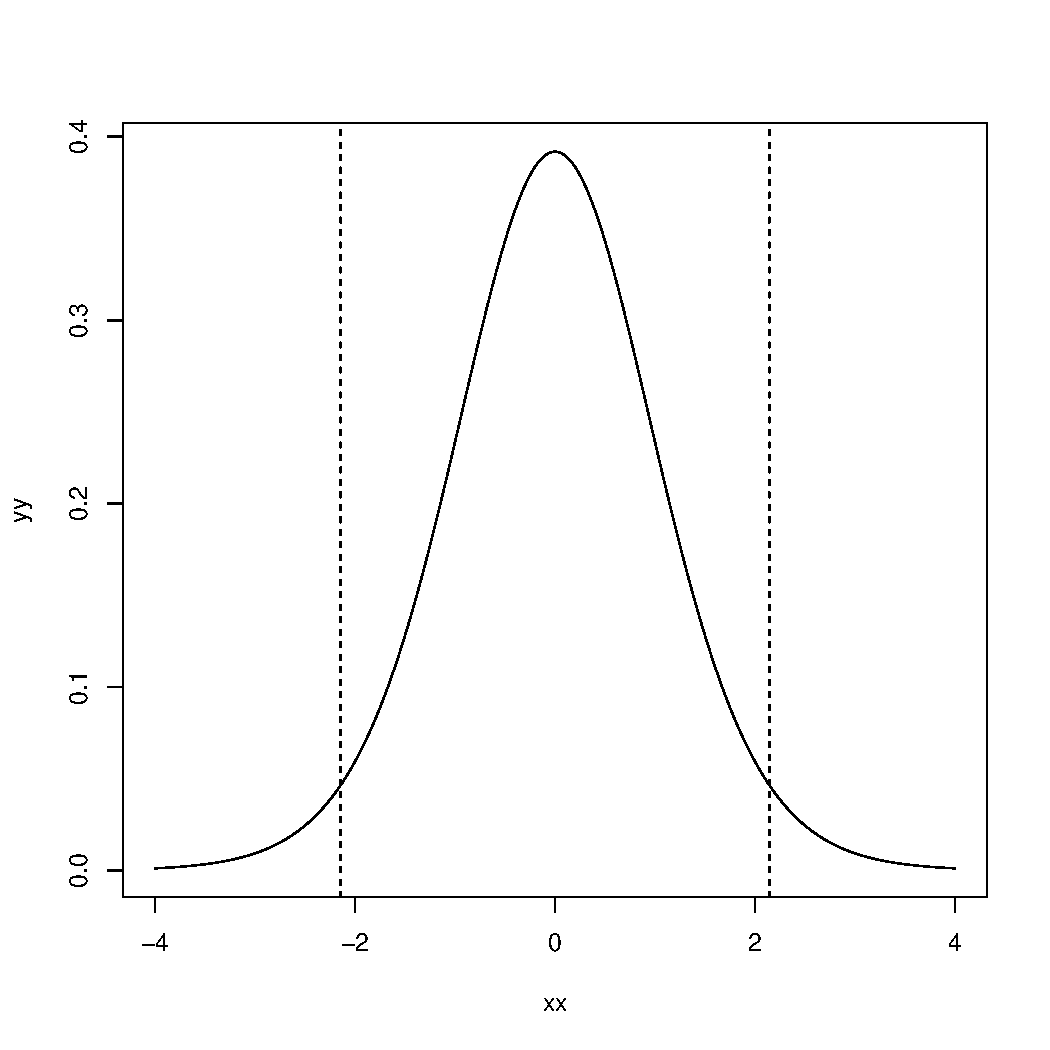
\includegraphics[width=\maxwidth]{figure/unnamed-chunk-12-1} 

\end{knitrout}

    \item Fail to reject $H_0$ since $|t| = 1.161895$ is not in the rejection region.

  \end{enumerate}
  
  \item[Problem 2] The correct answer is b) (since $0.01 < p \le 0.05$).
  
  \item[Problem 4]
  
  \begin{enumerate}
  
    \item The correct answer is that $n$ will go UP!
    
    \item The correct answer is that $n$ will go DOWN!
    
    \item The correct answer is that $n$ will go UP!
  
  \end{enumerate}

  \item[Problem 6] Here, $\mu$ is the mean level of serum acid phosphatase in prostate cancer patients where the cancer has spread to surrounding lymph nodes. We wish to test the hypothesis
  \begin{equation*}
    H_0: \mu = 0.645 \quad vs. \quad H_1: \mu > 0.645
  \end{equation*}
The observed $t$-statistic is 2.5616 and the observed significance level (i.e., the $p$-value) is 0.009542. Hence, we would reject the null hypothesis at the 0.05 level of significance and conclude that the mean level of serum acid phosphatase in prostate cancer patients where the cancer has spread to surrounding lymph nodes is elevated.

\end{description}

\end{document}
